\section{The Large Hadron Collider and the ATLAS experiment}\label{sec:LHC and ATLAS}
%\pagestyle{plain}

A brief introduction to the physics investigated at the Large Hadron Collider (LHC)\cite{lhc}, its design and the ATLAS\cite{atlas1,atlas2} experiment is provided in this chapter.

\subsection{Physics at the LHC}

The LHC goal is to help answering some of the fundamental open questions in particle-physics. The basic laws governing the interactions and forces among the elementary objects and the interrelation between quantum mechanics and general relativity are the main questions that LHC wants to address.\\
The discovery of the Higgs boson was one of the principal target of the LHC, as well as detailed studies about its properties. The Higgs boson was the last missing block to the validation of the Standard Model theory\cite{SM1,SM2,SM3} as it will be explained in the next section.
Data is also needed from high energy particle experiments to suggest which versions of the current theoretical models are more likely to be correct. Many theories \cite{theories} expect new physics beyond the Standard Model to emerge at the LHC energy level. %as the Standard Model appears to be unsatisfactory. % Issues possibly to be explored by LHC collisions include:[16][17]


\subsubsection{The Standard Model}

\label{sect:standard_model}
The Standard Model (SM) of particle physics attempts to describe, on the most basic level, the particle structure of matter and their interactions via the fundamental forces.
The SM describes three of the four fundamental forces (electromagnetic, weak and strong) in terms of a quantum field theory in which the Lagrangian is invariant under a continuous group of local transformations, a gauge theory \cite{gauge-theory}.\\
%The SM is based on a symmetry group of the kind $SU(3)_C\otimes SU(2)_I\otimes U(1)_Y$, this means that the SM Lagrangian is invariant under each of the group, where $SU(3)_C$ describes the coulour C symmetry of strong interaction, $SU(2)_I$ describes the weak isospin I for unified electro-weak interactions and $U(1)_Y$ the invariance under hyper-charge Y transformations.
%In particular the SM unifies the description of the electromagnetic and weak force in the $SU(2)_I\otimes U(1)_Y$ symmetry group, the electro-weak symmetry.\\
Within the SM all matter consists of a finite irreducible set of spin-$\frac{1}{2}$ particles denoted as fermions \index{fermion} that interact via the exchange of bosons\index{boson}, particle which are defined by their integer spin. Two different type of bosons are present in the SM, gauge bosons and scalar bosons.\\% The bosons in the theory act as the force carriers for the electro-weak and strong forces.\\ 
The fermions are subdivided into leptons and quarks, depending on their electric charge and their ability to interact with the strong force.
Leptons are observed to exist with integer or null electric charge as defined in units of the charge of the electron. There are three flavors of leptons forming a progressive mass hierarchy in a doublet \index{lepton!flavor!doublets} arranged structure whereby each charged lepton is associated with a zero-mass, neutrally-charged one denoted as a neutrino,
\begin{equation}
\label{eqn:lepton_flavor_doublets}
\begin{pmatrix} e       \\ \nu_e      \end{pmatrix} \qquad
\begin{pmatrix} \mu     \\ \nu_{\mu}  \end{pmatrix} \qquad
\begin{pmatrix} \tau    \\ \nu_{\tau} \end{pmatrix}
\end{equation}
%
The three charged leptons, the electron, the muon, and the tau ($e^-$, $\mu^-$ and $\tau^-$) each with negative charge are taken as the base particles states, while their charge conjugates are denoted as their anti-particles states.  Within the SM there exists no mechanism which, in a direct fashion, provides for horizontal mixing between the \index{lepton!family} \index{lepton!horizonal mixing} lepton families; as a result members of each family are assigned a \index{lepton!lepton number} quantum number $L_{\ell}$ corresponding to the lepton flavor of the particle.
%%%%%%%%%%%%%%%%%%%%%%%%
% Begin Table Block
\begin{table}
	\begin{center}
		\begin{tabular}{|c|c|c| c c c|}
			\hline
				Lepton        & Mass           & Charge & $L_{e}$ & $L_{\mu}$ & $L_{\tau}$ \\
			\hline
				$e^{-}$      & $0.51 \mbox{ MeV}$     & $-1 e$ & 1       & 0         & 0 \\
				$\mu^{-}$    & $105.65 \mbox{ MeV}$   & $-1 e$ & 0       & 1         & 0 \\
				$\tau^{-}$   & $1777.03 \mbox{ MeV}$  & $-1 e$ & 0       & 0         & 1 \\
			\hline
				$\nu_{e}$    & $< 3 \mbox{ eV}$       & $0$    & 1       & 0         & 0 \\
				$\nu_{\mu}$  & $< 0.19 \mbox{ MeV}$   & $0$    & 0       & 1         & 0 \\
				$\nu_{\tau}$ & $< 18.2 \mbox{ MeV}$   & $0$    & 0       & 0         & 1 \\
			\hline
		\end{tabular}
		\caption{Lepton Properties~\cite{PDG}}
		\label{table:lepton_properties}
	\end{center}
\end{table}
% End Table Block
The mass hierarchy of the lepton doublets is clear from Table~\ref{table:lepton_properties}.\\
The distinguishing feature of the leptons is that they do not experience a direct interaction with the strong nuclear force. All lepton interactions occur through \index{electro-weak interactions} electro-weak interaction couplings. \\%, shown in Fig.~\ref{fig:lepton_electro_weak}, and as such are a sensitive probe into the structure of the \index{weak current} weak currents.
In contrast to leptons, quarks are distinguished by their interactions with the strong nuclear force and their fractional electric charge. Strong force \index{strong force} \index{quark!confinement} binding and confinement lead quarks to form the fundamental substructure for all hadronic matter. Two types of structure are framed, either a color neutral three-quark bound state that form the common baryons such as the proton and neutron, or a quark-antiquark bound state mesons such as the $\pi,K,\eta$, and $\rho$. Free quarks are not accessible due to the requirements of color neutrality, which require a stable state to have a net color charge of 0, leading to the so called color confinement. The typical range of strong interaction is $\sim$\SI{e-15}{\meter}\\
Similarly to the leptons, there exists a generational hierarchy of distinct quark flavor doublets \index{quark!flavor!doublets} based on the masses of each quark and their asssociated quantum properties. Each generation consists of two quarks each with fractional electric charges equal to $-\frac{1}{3}$ and $\frac{2}{3}$ the charge magnitude of the electron. There exists evidence for three such quark generations whose associated quarks we label as up, down, charm, strange, top, bottom.  They are arranged in flavors doublets as: \index{quark!up|see{up quark}} \index{quark!down|see{down quark}} \index{quark!strange|see{strange quark}} \index{quark!charm|see{charm quark}} \index{quark!top|see{top quark}} \index{quark!bottom|see(bottom quark)} \index{up quark} \index{down quark} \index{strange quark} \index{charm quark} \index{top quark} \index{bottom quark}

\begin{equation}
\begin{pmatrix} u \\ d \end{pmatrix} \qquad
\begin{pmatrix} c \\ s \end{pmatrix} \qquad
\begin{pmatrix} t \\ b \end{pmatrix}
\label{eqn:quark_flavor_doublets}
\end{equation}

The mass hierarchy of the quark doublets is clear from Table~\ref{table:quark_properties}. As with the leptons, each quark flavor has a corresponding anti-particle state leading to a total of 12 distinct particles. These quarks have strong, weak, and electro-magnetic interactions. Unlike the lepton sector, the weak interaction vertex can mix quark \index{quark!mixing} flavors between generations leading to $s \rightarrow u$ like processes arising via weak currents. \index{weak current}

As previously said the SM describes the fermions interaction by the use of bosons. Two types of bosons are present in the SM: the gauge bosons (or vector bosons) and the scalar bosons.
Gauge bosons are distinguished by their spin-1, they are responsible of the fundamental interaction. Photons describe the electromagnetic interactions, the $W^\pm$ and the $Z$ describe the weak interaction while the gluons, which could have 8 different color state, describe the strong interaction.
Photons and gluons are massless while $W^\pm$ and $Z$ have respectively a mass of ($80.403 \pm 0.029$) \GeV \cite{PDG} and ($91.1876\pm0.021$) \GeV \cite{PDG}; due to their mass the range of interaction of weak force is short: typically $\sim\SI{e-18}{m}$. %Strong force has as well a short interaction distance due to the confinement property of Quantum Chromo Dynamics (QCD).
Photons are massless and not subject to QCD behavior, so that the interaction distance of electromagnetic force is not limited.

The only scalar boson present in the SM is the Higgs boson. The role of the Higgs boson is strictly connected to the SM mathematical structure.
The mass of the particles is generated in the SM by the introduction of a scalar field in the SM Lagrangian, this operation is known as electroweak symmetry breaking (EWSB).
The Higgs boson discovery was announced on $4^{th}$ of July 2012 by the ATLAS and CMS experiment at LHC and it is measured to have a mass of $m_H=125.09\pm0.21(stat.)\pm0.11(syst.) \GeV$ \cite{higgs_mass}. 

%%%%%%%%%%%%%%%%%%%%%%%%%%%
%%%%%%%%%%%%%%%%%%%%%%%%%%%

%%%%%%%%%%%%%%%%%%%%%%%%
% Begin Table Block
\begin{table}
\begin{center}
\begin{tabular}{|c|c|c|c|}
\hline
Quark & Mass & Charge & Properties \\
\hline
u & $1-5 \mbox{ MeV/c}^2$         & $\phantom{-}\frac{2}{3} e$  & $I_{z} = \frac{1}{2}$ \\
d & $3-9 \mbox{ MeV/c}^2$         & $-\frac{1}{3} e$ & $I_{z} = -\frac{1}{2}$ \\
c & $1.15-1.35 \mbox{ GeV/c}^2$   & $\phantom{-}\frac{2}{3} e$  & Charm = +1 \\
s & $75-170 \mbox{ MeV/c}^2$      & $-\frac{1}{3} e$ & Strangeness = -1 \\
t & $\approx 174 \mbox{ GeV/c}^2$ & $\phantom{-}\frac{2}{3} e$  & Top = +1 \\
b & $4.0-4.4 \mbox{ GeV/c}^2$     & $-\frac{1}{3} e$ & Bottom = -1 \\
\hline
\end{tabular}
\caption{Quark Properties}
\label{table:quark_properties}
\end{center}
\end{table}

% End Table Block
%%%%%%%%%%%%%%%%%%%%%%%%
\index{standard model|)}

%%% Local Variables: 
%%% mode: latex
%%% TeX-master: "section_wrapper"
%%% End: 

%\subsubsection{The Standard Model and the Higgs Boson}
%The Standard Model (SM) is a quantum field theory that provides a description of matter at subnuclear level and of three of the four fundamental interaction: the electromagnetic, the weak and the strong force.
%The description of matter and interaction is provided by the concept of particles, objects with no internal structure defined by their quantum numbers.\\

%Two categories of particles are present in the SM: fermions, particles with spin-$\frac{1}{2}$, and bosons, particles with integer spin.
%Fermions are the basic constituents of matter, they divide in leptons and quarks.
%The SM hosts six leptons and six quarks, for each of them it foreseen a respective anti-particle. Fermions are the building block of matter.
%The six leptons are organized in three family
%\begin{table}
%\center
%\end{table}
%Bosons can have in the SM either spin-1 or spin-0. Bosons that have spin-1 are the one describing an interaction and they are also said vector bosons or gauge bosons.
%There is only one particle with spin-0 and it is the Higgs boson.

\subsubsection{Physics beyond the Standard Model}

%- Why the SM is not definitive?
%The SM of particle physics describes the known phenomena below an energy scale of the order of 100 GeV.
%The SM has been object of detailed experimental studies and it has been demonstrated to give a precise description of the particle physics phenomena up to the \TeV energy scale, i.e. at the Tevatron\cite{Tevatron}. The SM needs to be tested to larger energy scale and this is one of the purposes of the LHC.\\
Even though the SM has proven to give a precise description of the particle physics up to the \TeV~scale, there are several unsolved question that the it does not answer.\\
\begin{itemize}
\item The SM does not provide any description of the gravitational force and it does not provide a physics description at energies typical of Grand Unification Theory (GUT) or Planck scale.
\item The SM cannot explain the very large difference between the electroweak energy scale and the GUT or the Planck scales. This is called hierarchy problem. The hierarchy problem has a drawback in the estimation of Higgs vacuum field using a perturbative theory approach, leading to divergent contributions to the Higgs mass that are not cancelled.
\item Cosmological observations point out the need to include Dark Matter (DM) in the description of the universe. A successful DM candidate must be stable, electrically neutral, weakly interacting and massive (non-relativistic): this excludes any known Standard Model particle.
\item The SM describes neutrinos as massless. However the experimentally established phenomenon of neutrino oscillation, which mixes neutrino flavor states with neutrino mass states, requires neutrinos to have masses.
\item The SM does not provide any description of the observed matter-antimatter asymmetry.
\end{itemize}
All these open question lead to the idea that the SM is an effective theory that works fine at the electroweak scale, but is incomplete when it is extended to higher energies.\\
Several theoretical models have been developed for overcoming those issues; for example models that foreseen exotic particles\footnote{An exotic particle is a hypothetical particle foreseen by some theoretical models.} and Supersymmetry (SUSY). In SUSY each particle is associated with a particle not foreseen in the Standard Model, known as its super-partner, the spin of which differs by a half-integer. \\
The experiments at LHC are investigating several models within the exotic particle and SUSY hypothesis, which are potential candidates for new physics discovery. The LHC is investigating, as well, the asymmetry in matter-antimatter by studying the CP violation and looking for potential candidates for the explanation of the Dark Matter. 



\subsection{The Large Hadron Collider}

\label{sect:lhc}
%The LHC was installed in a \SI{26.7}{\kilo\meter} diameter tunnel, previously adopted by the Large Electron-Positron Collider (LEP)\cite{lep}.
The Large Hadron Collider (LHC)\cite{lhc} is a two-ring-hadron accelerator and collider which is located at CERN\footnote{CERN: the European Organization for Nuclear Research}. 
The LHC project started in the early '90 of the last century with the aim of building a collider able to deliver a center of mass energy at the scale of $\sim10$ TeV, an order of magnitude higher than the already existing hadronic collider (Tevatron) and two order of magnitude greater than the leptonic one (LEP).
The LHC is a hadronic collider that is used for proton-proton, heavy-ions and proton-heavy-ion collisions. Only  but  proton-proton collisions are considered in the work presented in this thesis.

\subsubsection{The advantages and challenges of hadron colliders}
The main motivation to use a hadron collider instead of electron-positron one, as it was LEP, is the much higher and wider achievable center of mass energy, which allows to investigate a higher energy and it suits better than a leptonic machine for potential discovery of new particles. Colliders which accelerate electrons are limited in energy due to synchroton radiation: which is the electromagnetic radiation generated by the acceleration of ultrarelativistic charged particles through magnetic fields. The energy loss in due to synchtron radiation is:
\begin{equation}
\label{eq:synchrad}
\frac{dE}{dt} \propto \frac{E^4}{m^4R}
\end{equation}
where E is the energy of the beam particles, m the mass, and R the bending radius.\\
There is another family of lepton colliders, the muon colliders, which at the moment is still at R\&D stage. Muon colliders does not suffer from synchtron radiation at TeV scale, given the previous formula. The challenge of muon colliders is represented by the limited lifetime of a muon at rest, $\sim2.2~\mu s$, which will be extended to few micro-seconds for muons at TeV energy. Muons must be produced and collected, cooled, and re-accelerated quickly. This forces many of the components to provide multiple functions, combining cooling, acceleration, and focussing. The beam transport system must handle the radiation and heat load associated with electrons from muon decay. Detectors must be well-shielded from the bulk of the decay backgrounds.\\
Hadron colliders do not suffer of energy leakage from synchrotron radiation at the TeV scale and they use stable particles, so that there are no time constrains in the preparation of the beam before the collisions. 
The choice of a hadron collider, instead of a leptonic, brings features related to the composite structure of the hadrons.
In hadron colliders the partonic center of mass energy is stochastic, making kinematic calculation more difficult with respect to leptonic ones. The composite structure of the hadrons is not only a drawback, at each collision the energy of the parton is  only a part of the energy of the hadron itself. This allow to scan a wide energy range without changing the beam configuration, differently from leptonic colliders.
Moreover the cross section for hard collisions, which have a large momentum transferred, is much smaller than the one for soft collisions, the ones where the protons interact as a whole object. Discovery of new physics can happen at the quark level, so that a hadronic machine has to operate with high collision rate, typically \SI{40}{\mega\hertz} for the LHC.\\
At the LHC the hard scattering events of interest will originate from a single proton-proton interaction out of the collision of two bunches filled with protons. While it is extremely unlikely that more than one colliding proton-proton pair will produce a high-pt hard scattering event when the collision of the two bunches takes place, in general several additional low-pt interactions will take place among other proton-proton pairs in the same bunch. These are usually called pile-up collisions and they are completely independent from the hard scattering process.
In addition to the in-time pile-up, where low-pt events come from interaction in the same bunch, also out-of-time pile-up events have to be considered. In fact the time interval between two consecutive collisions is \SI{25}{\nano\second}, which is shorter than the average time response of many of the detectors subsystems.
Finally the underlying event is defined as the outcome of additional parton interactions taking place among components of the same protons which give rise to the hard scattering process of interest. The additional parton-parton interaction result in a low-pt scattering process. 

\subsubsection{The LHC design}
\begin{figure}
\centering
\includegraphics[width=0.7\textwidth]{Images/atlas/lhc_injectors.png}
\caption{Injection chain of the LHC}
\label{fig:lhc_inj}
\end{figure}
The LHC consists of two rings with counter-rotating beams for hosting and accelerating hadrons, i.e. proton and lead nuclei. Due to the limited size of the hosting tunnel, a two-in-one design was chosen for the superconducting magnets so that the system provides a magnetic field in opposite direction for the two rings.
The acceleration chain of the LHC is schematized in Figure~\ref{fig:lhc_inj} and it consists of several stages. The proton source is a simple bottle of hydrogen gas. An electric field is used to strip hydrogen atoms of their electrons to yield protons. Linac 2, the first accelerator in the chain, accelerates the protons to the energy of \SI{50}{\MeV}. The beam is then injected into the Proton Synchrotron Booster (PSB), which accelerates the protons to \SI{1.4}{\GeV}, followed by the Proton Synchrotron (PS), which pushes the beam to \SI{25}{\GeV}. Protons are then sent to the Super Proton Synchrotron (SPS) where they are accelerated to \SI{450}{\GeV}.
The protons are finally transferred to the two beam pipes of the LHC. The beam in one pipe circulates clockwise while the beam in the other pipe circulates anticlock-wise. It takes 4 minutes and 20 seconds to fill each LHC ring, and 20 minutes for the protons to reach their maximum energy. Beams circulate for many hours inside the LHC beam pipes, then, when the population of proton decreases, the beam is dumped and a new fill of protons is performed from the SPS. The two beams are brought into collision inside four detectors: ALICE, ATLAS, CMS and LHCb. Lead ions for the LHC start from a source of vaporized lead and enter Linac 3 before being collected and accelerated in the Low Energy Ion Ring (LEIR). They then follow the same route to maximum energy as the protons.
The designed maximum beam energy that the LHC can deliver is $7\,\TeV$ per beam and it depends on nominal magnetic field $\sim8.33~T$ of the bending dipole magnets. Therefore the maximum energy in the center of mass for the LHC machine is $\sqrt{s} = 14\,\TeV$.
Another important parameter of particles colliders is the luminosity, defined as the ratio of the number of events detected (N) in a certain time (t) to the interaction cross-section ($\sigma$):

\begin{equation}
L = \frac{1}{\sigma}\frac{dN}{dt} = f \frac{n_1 n_2}{A_{eff}}
\end{equation}
where $n_1$ and $n_2$ are the number of particles contained in the two opposite orbiting bunches, $f$ is the collision frequency and $A_{eff}$ is the effective collision area. The size of collision area depends on the beam width in the horizontal ($\sigma_x$) and vertical ($\sigma_y$) axes. Under the assumption of gaussian beam $A_{eff} = 4\pi \sigma_x \sigma_y$.
Luminosity can be also express in terms of the geometrical characteristics of the colliding bunches and of the machine parameters as:
\begin{equation}
L = \frac{N^2_b n_b f_{rev} \gamma_r}{4\pi \epsilon_n \beta^*}F
\end{equation}
where $N_b$ is the number of particles per bunch, $n_b$ is the number of bunches per beam, $f_{rev}$ is the revolution frequency, $\gamma_r$ is the relativistic gamma factor, $\epsilon_n$ is the normalized tranverse beam emittance, $\beta^*$ is the distance from the interaction point at which the beam is twice as wide as the focus point and $F$ is the geometrical reduction factor due to the crossing angle at the interaction point .
\begin{equation}
F = \frac{1}{\sqrt{1 + ( \frac{\theta_c \sigma_z}{2\sigma^*} )^2}}
\end{equation}
where $\theta_c$ is the full crossing angle at the interaction point, $\sigma_z$ is the RMS of the bunch lenght and $\sigma^*$ is the RMS of the transverse beam size at the interaction point.
\begin{table}
\center

\begin{tabular}{lcc}
\hline
								& Injection & Collision\\%	& Run II initial paramaters \\
\hline
Energy 							& $450~GeV$  	& $7~TeV$ \\
Luminosity 						& & $10^{34}~cm^{-2}s^{-1}$  \\ %       &  \\
								& &  \\
Number of bunches 					& \multicolumn{2}{c}{2808}\\ 		%	  & $\simeq40$  \\
Bunch spacing 						& \multicolumn{2}{c}{25 | \SI{50} {\nano\second}}\\% & 50 ns \\
Number of particles per bunch 			& \multicolumn{2}{c}{$\simeq2\times 10^{11}$}       \\
Beam current 						& \multicolumn{2}{c}{\SI{0.58}{\ampere}} \\
Transverse emittance 				&\SI{3.5}{\micro\meter}	&\SI{3.75}{\micro\meter} \\
Longitudinal emittance 				& \SI{1.0}{\eV} 	& \SI{2.5}{\eV} \\
Synchtron radiation loss per turn		& \SI{0}{\eV} 	& \SI{7}{\keV} 	\\
Bunch lenght (4$\sigma$)				&\SI{1.7}{\nano\second} &\SI{1.0}{\nano\second} \\
Relativistic gamma 					& 479.6 & 7461 \\
$\beta$							& \SI{18}{\meter} & \SI{0.55}{\meter}\\
$\frac{\theta_c}{2}$ 					& $\pm$\SI{160}{\micro\radian}& $\pm$\SI{142.5}{\micro\radian} \\
Geometrical reduction factor $F$ 		& - & 0.836 \\
RMS bunch lenght 					& \SI{11.24}{\centi\meter}& \SI{7.55}{\centi\meter}\\
RMS beam size 					& \SI{375.2}{\micro\meter}& \SI{16.7}{\micro\meter} \\
\hline
\end{tabular}

\caption{Main machine parameters of the LHC collider in the proton proton collision mode}
\label{table:LHC_par}
\end{table}

The main accelerator parameters in the proton-proton operation mode are reported in table~\ref{table:LHC_par}, the parameters are shown for injections and collisions.
%In addition to the beam energy, another relevant parameter is the distribution of the interaction point position, usually denoted as beam spot 



% This creates the need for a high luminosity operating collider: the rate of the proton-proton interactions inside the LHC machine is given by the product of the proton-proton cross section $\sigma$ and the luminosity L.
%The instantaneous luminosity L, defined in equation , is the product of the numbers of particles $n_1$, $n_2$ in both crossing bunches and the frequency f of bunch crossings, divided by the cross sectional area $A = 4\pi \sigma _x \sigma _y$ of a bunch:



%Although in a lepton collider all the center of mass energy is given to two point object there are limitation to the maximum energy achievable due to synchrotron radiation, leading to a large energy. loss in $e^+e^−$colliders, is the crucial limiting factor. Charged particles moving along a curved
%trajectory loose energy following the relation:
%where E and m are particle’s energy and mass, while R is the trajectory’s radius of curvature. This implies that at fixed energy and collider dimensions (radius), electrons loose (mp/me)4 ∼ 1012 times more energy than a proton beam with the same characteristics. The use of electrons would have been possible only in a synchrotron with a much larger radius or in a linear accelerator implying a much greater cost than the solution adopted.
%L=f n1n2 (1.2) 4πσxσy
%The instantaneous luminosity has been progressively increased during operation, as shown in figure 1.1. In 2012, for each bunch crossing there were up to about
%
%The experimental setup 3 30 collisions that summed themselves to each interaction with large transverse
%momentum. This soft-collision background is usually called pile-up.








\subsection{The ATLAS experiment}
\label{sect:atlas}
ATLAS (A Toroidal LHC ApparatuS)\cite{atlas} is one of the seven particle detector experiments (ALICE, ATLAS, CMS, TOTEM, LHCb, LHCf and MoEDAL) constructed at the LHC.
ATLAS and CMS are the two general-purpose detectors, designed to exploit the LHC physics scenario addressing outstanding questions related to the existence of the Higgs particle or, more generally, the nature of the electroweak symmetry breaking and the existence of new particles which may be produced at the TeV scale.
% The experiment is designed to take advantage of the unprecedented energy available at the LHC and observe phenomena that involve highly massive particles which were not observable using earlier lower-energy accelerators. It is hoped that it will shed light on new theories of particle physics beyond the Standard Model.
ATLAS is 46 meters long, 25 meters in diameter, and weighs about 7000 tonnes.% ATLAS is located close to the Meyrin village, near Geneva, in Switzerland.
%The experiment is done by a collaboration involving roughly 3000 physicists from over 175 institutions in 38 countries.


The high-energy and luminosity delivered by the LHC produce collisions in the ATLAS detector at high interaction rate, with very high radiation doses, in particular in proximity of the interaction region, where processes with high particle multiplicities and energies are produced. The search of the Higgs boson and for the new physics phenomena posed the following requirements:

\begin{itemize}
\item large geometrical acceptance with almost full azimuthal angle coverage;
\item good charged particle resolution and reconstruction efficiency;
\item good impact parameter resolution for jet coming from b-quarks and $\tau$ lepton identification, which requires vertex detector close to the interaction region despite the high radiation doses;
\item a very good electromagnetic calorimeter for electron and photon identification and measurements, complemented by a full-coverage hadronic calorimeter for accurate jet and missing transverse energy measurements;
\item  a precise muon identification and momentum resolution over a wide range of momenta;
\item a flexible and fast trigger system to select physically interesting events, even in the presence of low transverse-momentum objects and large background for uninteresting events.
\end{itemize}

In ATLAS, the nominal interaction point is defined as the origin of the coordinate system, the beam direction defines the \textit{z} axis. The positive \textit{x} direction is defined as pointing from the interaction region to the centre of the LHC ring.
The azimuthal angle $\phi$ is measured around the beam axis, while the polar angle $\theta$ is the angle from the beam axis. Usually the angle $\theta$ is more conveniently expressed in terms of the pseudo-rapidity $\eta = -ln(tan(\theta /2))$, which can be as well expressed in terms of momentum:

\begin{equation}
\label{eq:pseudorapidity}
 \eta = -\frac{1}{2}log(\frac{|\overrightarrow{p}|+p_L}{|\overrightarrow{p}|-p_L}).
\end{equation}

There are two arguments in favour of the use of pseudorapidity, for ultrarelativistic particle the definition of pseudorapidity is close to the rapidity, differences of rapidity are invariant under Lorentz boost.

\begin{equation}
y = -\frac{1}{2}log(\frac{E+p_L}{E-p_L}).
\end{equation}
As a consequence of the invariance of Lorentz boost, the production of particles at collider is flat in rapidity and it can be considered flat in pseudorapidity.\\
\begin{figure}
\center
\includegraphics[width=0.9\textwidth]{Images/atlas/ATLAS.jpg}
\caption{A three-dimensional view of the ATLAS detector}
\label{pic:atlas}
\end{figure}

The overall ATLAS detector layout is shown in Figure \ref{pic:atlas}. The main sub-detectors extend radially starting from the interaction point.
The closest detector to the interaction point is the Inner Detector, which is immersed in a 2T solenoidal field and which has a coverage up to $|\eta |\le 2.5$.
Outside the Inner Detector, the electromagnetic calorimeter, based on LAr technology, covers the pseudo-rapidity range up to $|\eta |\le 3.2$.
Behind it, the hadronic calorimetry is provided by scintillator-tile calorimeter in $|\eta |\le 1.5$ and by LAr technology up to $|\eta |\le 4.9$.
The muon spectrometer surrounds the calorimeter and has three layers of high precision tracking chambers, which extends up to $|\eta |\le 2.7$.
%A detailed description of the ATLAS detector can be found in the technical desing report (TDR), \cite{cit:atlas_tdr}.

\subsubsection{The magnet system}

The ATLAS magnet system\cite{atlas_magnet} configuration comprises a thin superconducting solenoid surrounding the Inner Detector cavity and three large superconducting toroids (one barrel and two end-caps), arranged with an eight-fold azimuthal symmetry around the calorimeters, which provide bending power for the muon spectrometer.
% The magnet system is shown in figure \ref{pic:magnet}
%
%\begin{figure}
%\center
%\includegraphics[width=0.7\textwidth]{Images/atlas/MAGNET.png}
%\caption{Schematic view of the ATLAS magnet}
%\label{pic:magnet}
%\end{figure}
The solenoid has its field axis matching the beam direction. It is made of a single-layer aluminum coil wound by a NbTi conductor, optimizing thus its thickness in order to have a small impact on the energy measurement in the calorimeters. The solenoid has an inner radius of \SI{1.23}{\meter} and a total length of \SI{5.8}{\meter}. A magnetic field of \SI{2}{\tesla} is produced in the central region of the the Inner Detector.
The external toroidal magnets use coils consisting of a conductor made of a mixture of aluminum, niobium, titanium and copper, and they extend the magnet system to a total of \SI{26}{\meter} length and \SI{20}{\meter} diameter. This configuration provides a magnetic field for the muon spectrometer of \SI{0.5}{\tesla} and \SI{1}{\tesla} in the barrel and end-caps, respectively. %The magnet system operates with nominal currents of \SI{8}{\kilo \ampere} for the solenoid, and of \SI{25}{\kilo\ampere} for the toroids, respectively. Every toroid has a separate cryogenic system, while in the end-caps the coils have common cryostat.


\subsubsection{Inner Detector}
The ATLAS Inner Detector\cite{atlas_id1,atlas_id2} (ID) is the detector system closer to the interaction point which is composed of three sub-detectors: a Pixel Silicon Detector (Pixel), a Silicon Micro-Strip Detector (SCT) and a Transition Radiation Tracker (TRT).
Aim of the ID is the reconstruction of charged tracks, in terms of momentum and impact parameters. This reconstruction is achieved by combining the energy hits deposited in each of its sub-detector. The layout of the ID is illustrated in Figure \ref{pic:id}.
Since this thesis is mainly focused on the Pixel Detector upgrade, a detailed description of the ATLAS Pixel detector is given in Section~\ref{sec:pixel}, while brief descriptions of the silicon micro-strip detectors and of the transition radiation tracker follows.
\begin{figure}
\center
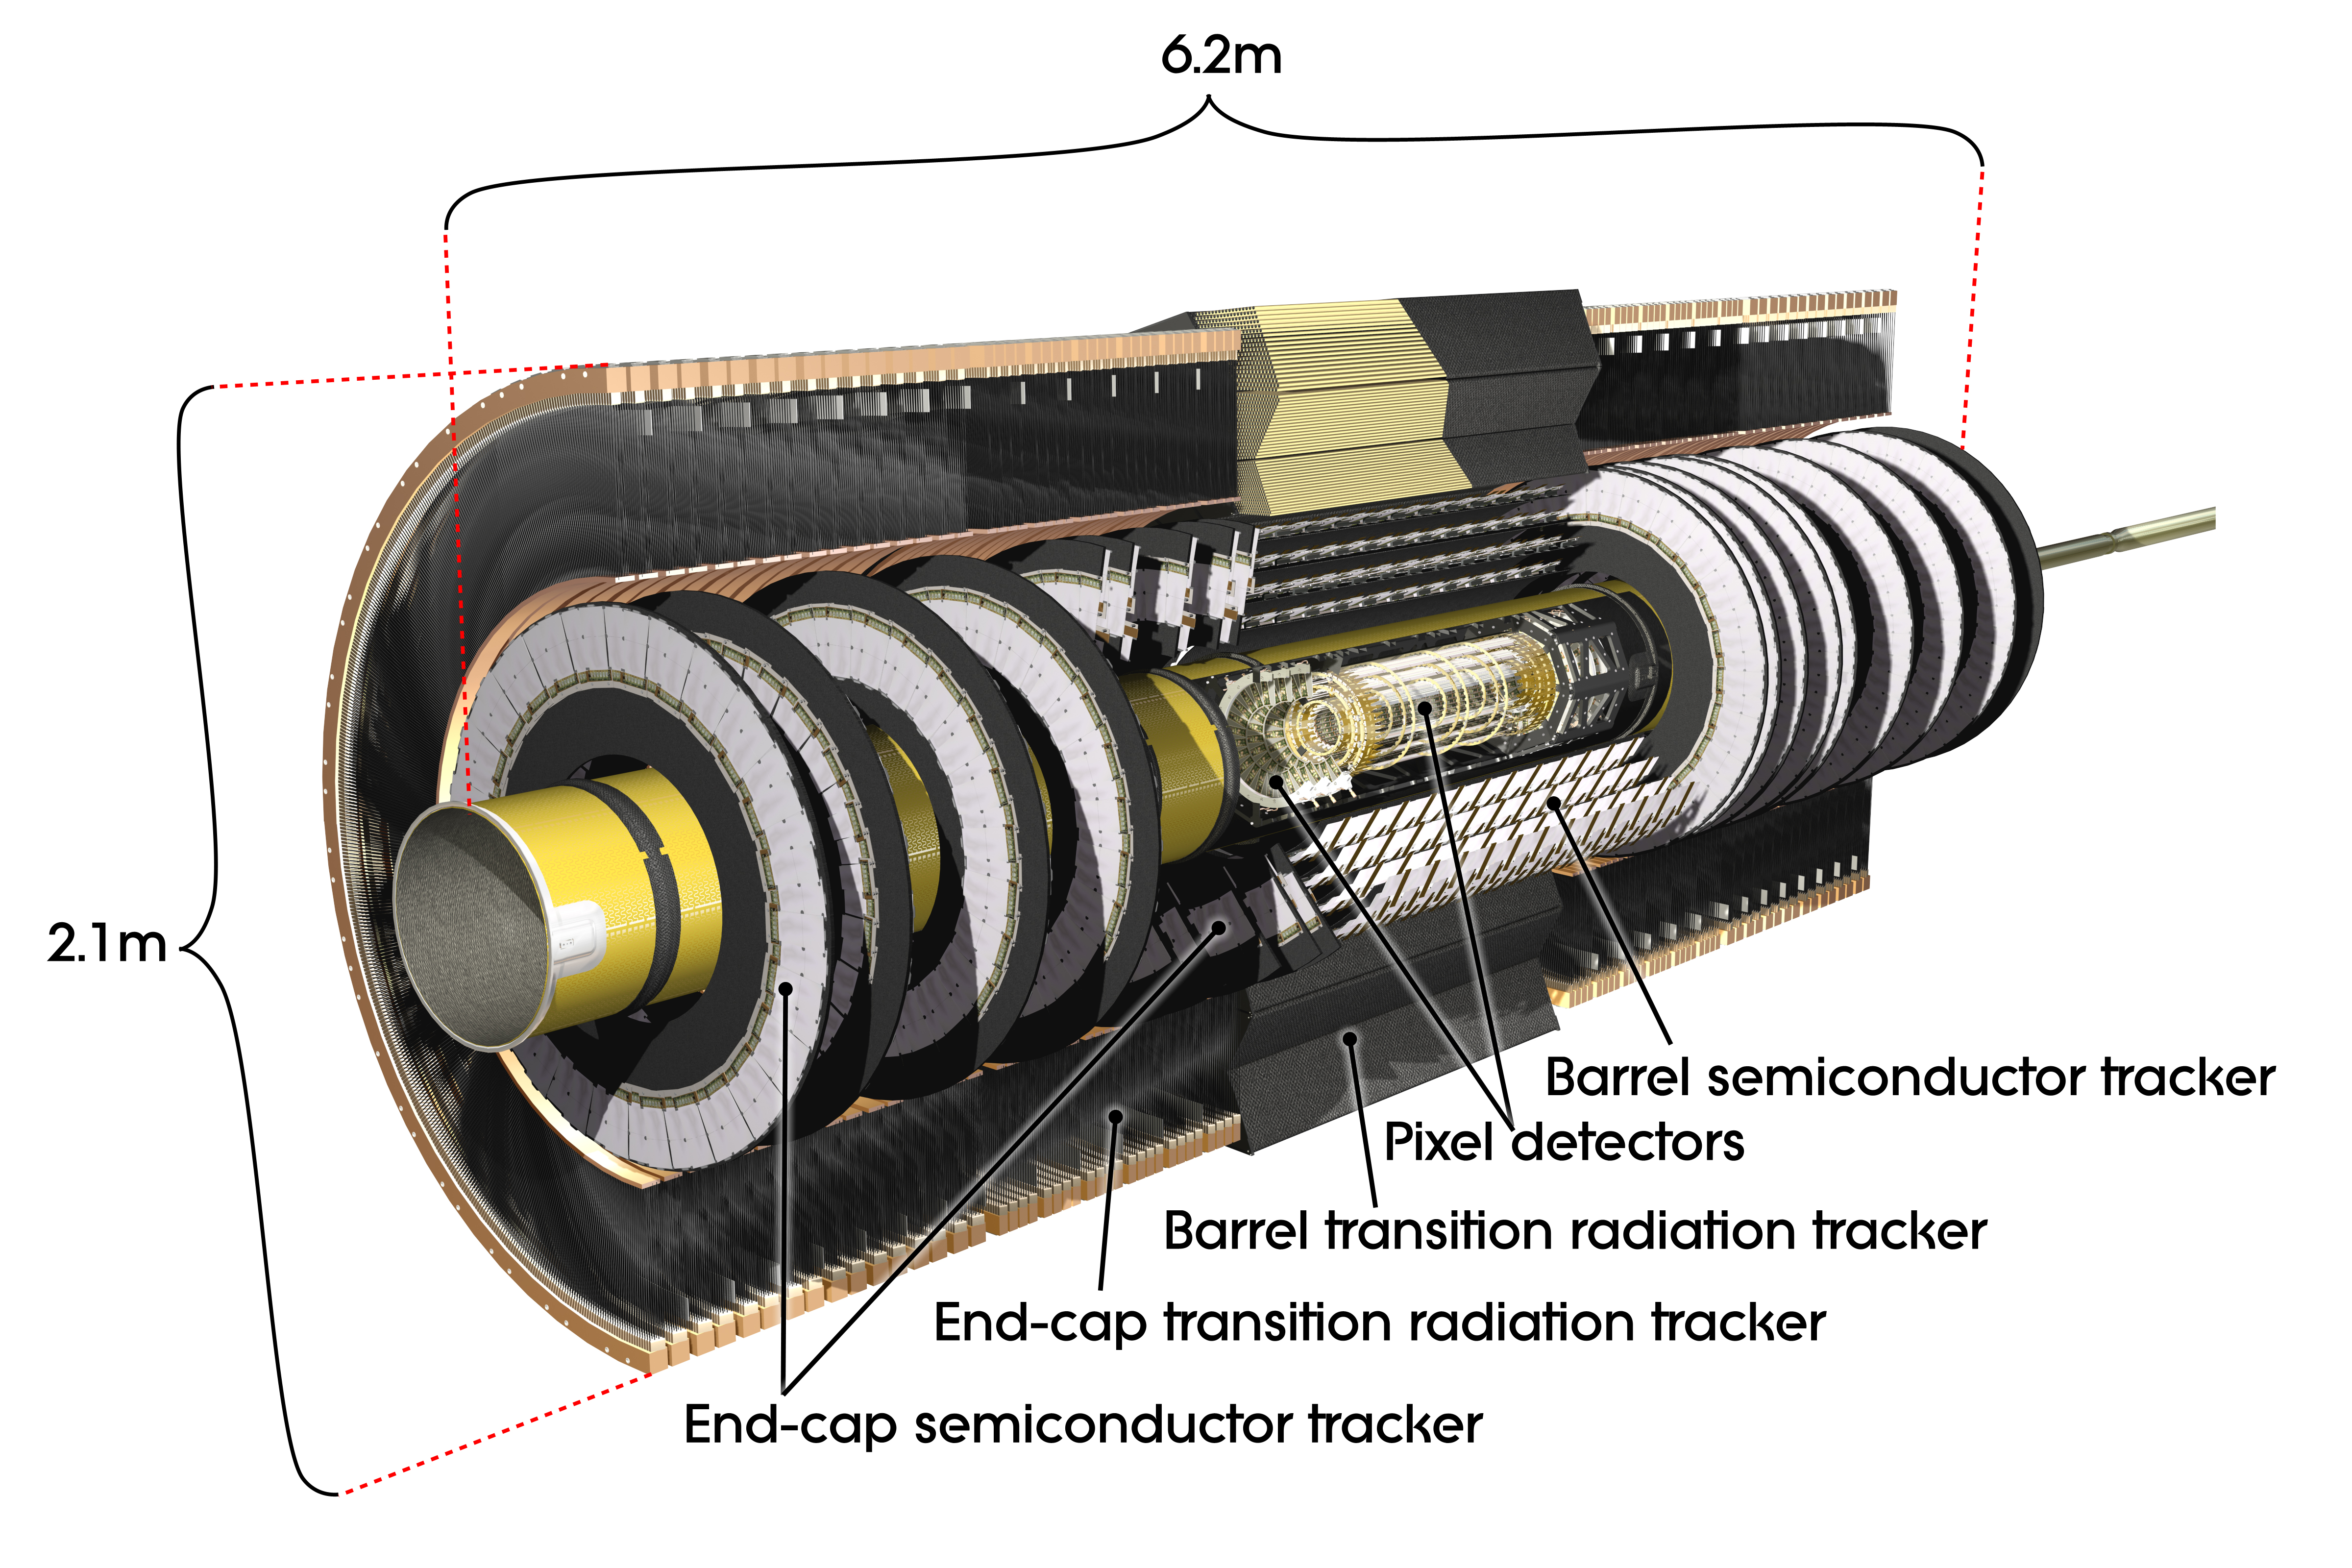
\includegraphics[width=0.7\textwidth]{Images/atlas/ID.jpg}
\caption{Cut-away view of the ATLAS Inner Detector}
\label{pic:id}
\end{figure}

\paragraph{Silicon microstrip detector}
The SCT\cite{atlas_sct} consists of four nested cylindrical barrels in the centre and nine disks in each of the two end-caps. The barrels cover a region from 300 to \SI{520}{\milli\meter} in radius and have an active length of \SI{1530}{\milli\meter}, centered around the interaction point. The respective barrel layers are fully covered by 32, 40, 48 and 56 rows of twelve identical modules, overlapping in a tile-structure in order to ensure full coverage, making a total of 2112 modules. The end-caps consist of nine disks each placed in Z at $835$ to \SI{2788}{\milli\meter} and radii ranging from 259 to \SI{560}{\milli\meter}, with the modules being placed in three rings overlapping azimuthally, two on one side, one on the other, in order to achieve full coverage.
The SCT barrel modules are made of four sensors, glued in pairs on either side of a thermally conductive baseboard. The sensors are approximately 6$\times$\SI{6}{\square\centi\meter} p-in-n silicon wafers of approximately \SI{300}{\micro\meter} thickness. Each sensor has 768 strips with \SI{80}{\micro\meter} pitch. The end-cap modules are made of two or four wedge-shaped sensors of varying size depending on their position on the end-caps rings. The strip pitch varies from \SI{57}{\micro\meter} on the inner edge of the innermost sensors to \SI{94}{\micro \meter} on the outer edge of the outermost sensors. The top and bottom sensors are rotated by a stereo angle of \SI{40}{\milli\radian} with respect each other in order to obtain two-dimensional position information while keeping the number of ghost hits small. The strips in the barrel are oriented in Z-direction and radially in the end-caps in order to obtain the best position resolution in azimuthal direction.
 The intrinsic accuracy in the barrel region is \SI{17}{\micro\meter} ($R-\phi$) and \SI{580}{\micro\meter} (z). The total number of readout channels of the SCT is approximately 6.3 million.

\paragraph{Transition radiation tracker}
The TRT\cite{atlas_trt} is composed of \SI{1.43}{\meter} long cylindrical barrel layer ranging from 56 to \SI{108}{\centi\meter} in radius and two end-caps ranging from \SIrange{0.84}{2.71}{\meter} in z and \SIrange{64}{103}{\centi\meter} in radius.
Both parts contain similar carbon-polyimide straw tubes of \SI{4}{\milli\meter} in diameter  which are aluminium-coated on theri inner surface to form a cathode and contain a gold-plated tungsten wire of \SI{30}{\micro\meter} in diameter that is used as anode. The straws are filled with 70\percent Xe, 27\percent CO$_2$ and 3\percent O$_2$, the first component being the main gas in which ionisation occurs and the latter had to be added to avoid etching problems with the glass joins that holds the wires. The straws are operated in proportional mode with the electrodes being on $\sim$\SI{1500}{\volt} bias. The 52544 straws in the barrel are \SI{144}{\centi\meter} long and formed to modules in which they are embedded in polypropylene radiator foils in which transition radiation is produced.
Relativistic particles emit transition radiation when crossing the boundary of radiator foils which is subsequently detected in the straw tubes. The signal charge from particles traversing the straws of approximately \SI{2}{\keV} is significantly lower than the signal charge created by absorption of the transition radiation photons $\sim$ \SI{10}{\keV}. Since the intensity of the emitted radiation depends on the $\gamma = E/m$ of the particle, light particles will emit more transition radiation than heavier particles which is used in the TRT to distinguish electrons from other particles such as $\pi$-mesons.
While the intrinsic resolution of the TRT cannot compete with the resolution od the silicon based technology, the high number of measurements and the long lever arm with respect to the measurements in the silicon layers makes the TRT significantly contributing to the momentum resolution. In addition, the low detector granularity is compensanted by the larger  radial positions of the straw tubes, so that a standalone pattern recognition is still possible for instantaneous luminosities up to and not beyond the nominal luminosity of \SI{e34}{\per\square\centi\meter\per\second}.

\paragraph{Impact of detector material}
\begin{figure}
\centering
\includegraphics[width=0.8\textwidth]{Images/atlas/IDMatX0.png}
\caption{Material distribution ($X_0,\lambda$) at the exit of the ID envelope, including the services and thermal enclosures. The distribution is shown as a function of $\eta$ and averaged over $\phi$. The breakdown indicates the contributions of external services and of individual sub-detectors, including services in their active volume.}
\label{fig:matbud_x0}
\end{figure}
The material budget of the tracking system must be kept to a minimum in order to limit disturbing effects form multiple scattering and not desired interactions.
%The need of a high granularity tracking detectors, in particular in the proximity of the interaction region, with related electronics, readout services and cooling, results in a relatively heavy inner detector (more than 4 tonnes), with a quite significant material budget (which can be expressed in terms of radiation lenghts $X_0$ or interaction lenghts $\lambda$).
This material has been accurately mapped and introduced in the ATLAS simulation since the impact on ATLAS performance is expected to be large:

\begin{itemize}
\item a significant fraction of low energy pions will undergo inelastic hadronic interaction inside the inner detector volume
\item approximately 40\percent of the photons convert into an electron-position pair before reaching the LAr cryostat and the electromagnetic calorimeter
\item many electrons lose a good part of their energy through bremmstrahlung before reaching the calorimeter.
\end{itemize}

The first two effects will be an important factor limiting the b-jet identification performance. This relies in fact on distinguishing higher impact parameter tracks (from b-decays) from prompt tracks.
A description of material budget can be given in term of radiation length, $X_0$. This is a characteristic of a material, related to the energy loss of high energy, electromagnetic-interacting particles with it. The definition of X$_0$ is the mean length (in \SI{}{\centi\meter}) to reduce the energy of an electron by the factor 1/e. The X$_0$ can be calculated given the characteristics of the material:
\begin{equation}
X_0=\frac{716.4 \cdot A}{Z(Z+1)ln{\frac{287}{\sqrt{Z}}}}g\cdot cm^{-2}
\end{equation}
where Z is the atomic number and A is a mass number of the nucleus.
Figure~\ref{fig:matbud_x0} shows the estimation of the $X_0$ obtained in simulation by the probability to create a photo-conversion $\gamma\rightarrow e^- e^+$ interacting with the ID material. It is a result of the need to have cooling, services and electronics inside the detector volume in order to cope with the finely granulated tracking detector elements. 

\subsubsection{Calorimeter}

The requirement of hermeticity, which is a necessary condition to achieve good resolution of the measurement of the missing transverse momentum, is one of the key design components of the ATLAS calorimeter, which in fact has a coverage up to |$\eta$| = 4.9. Different technologies are used across different regions in pseudo-rapidity as the different calorimeter sub-detectors as Figure \ref{pic:calo} shows.

\begin{figure}
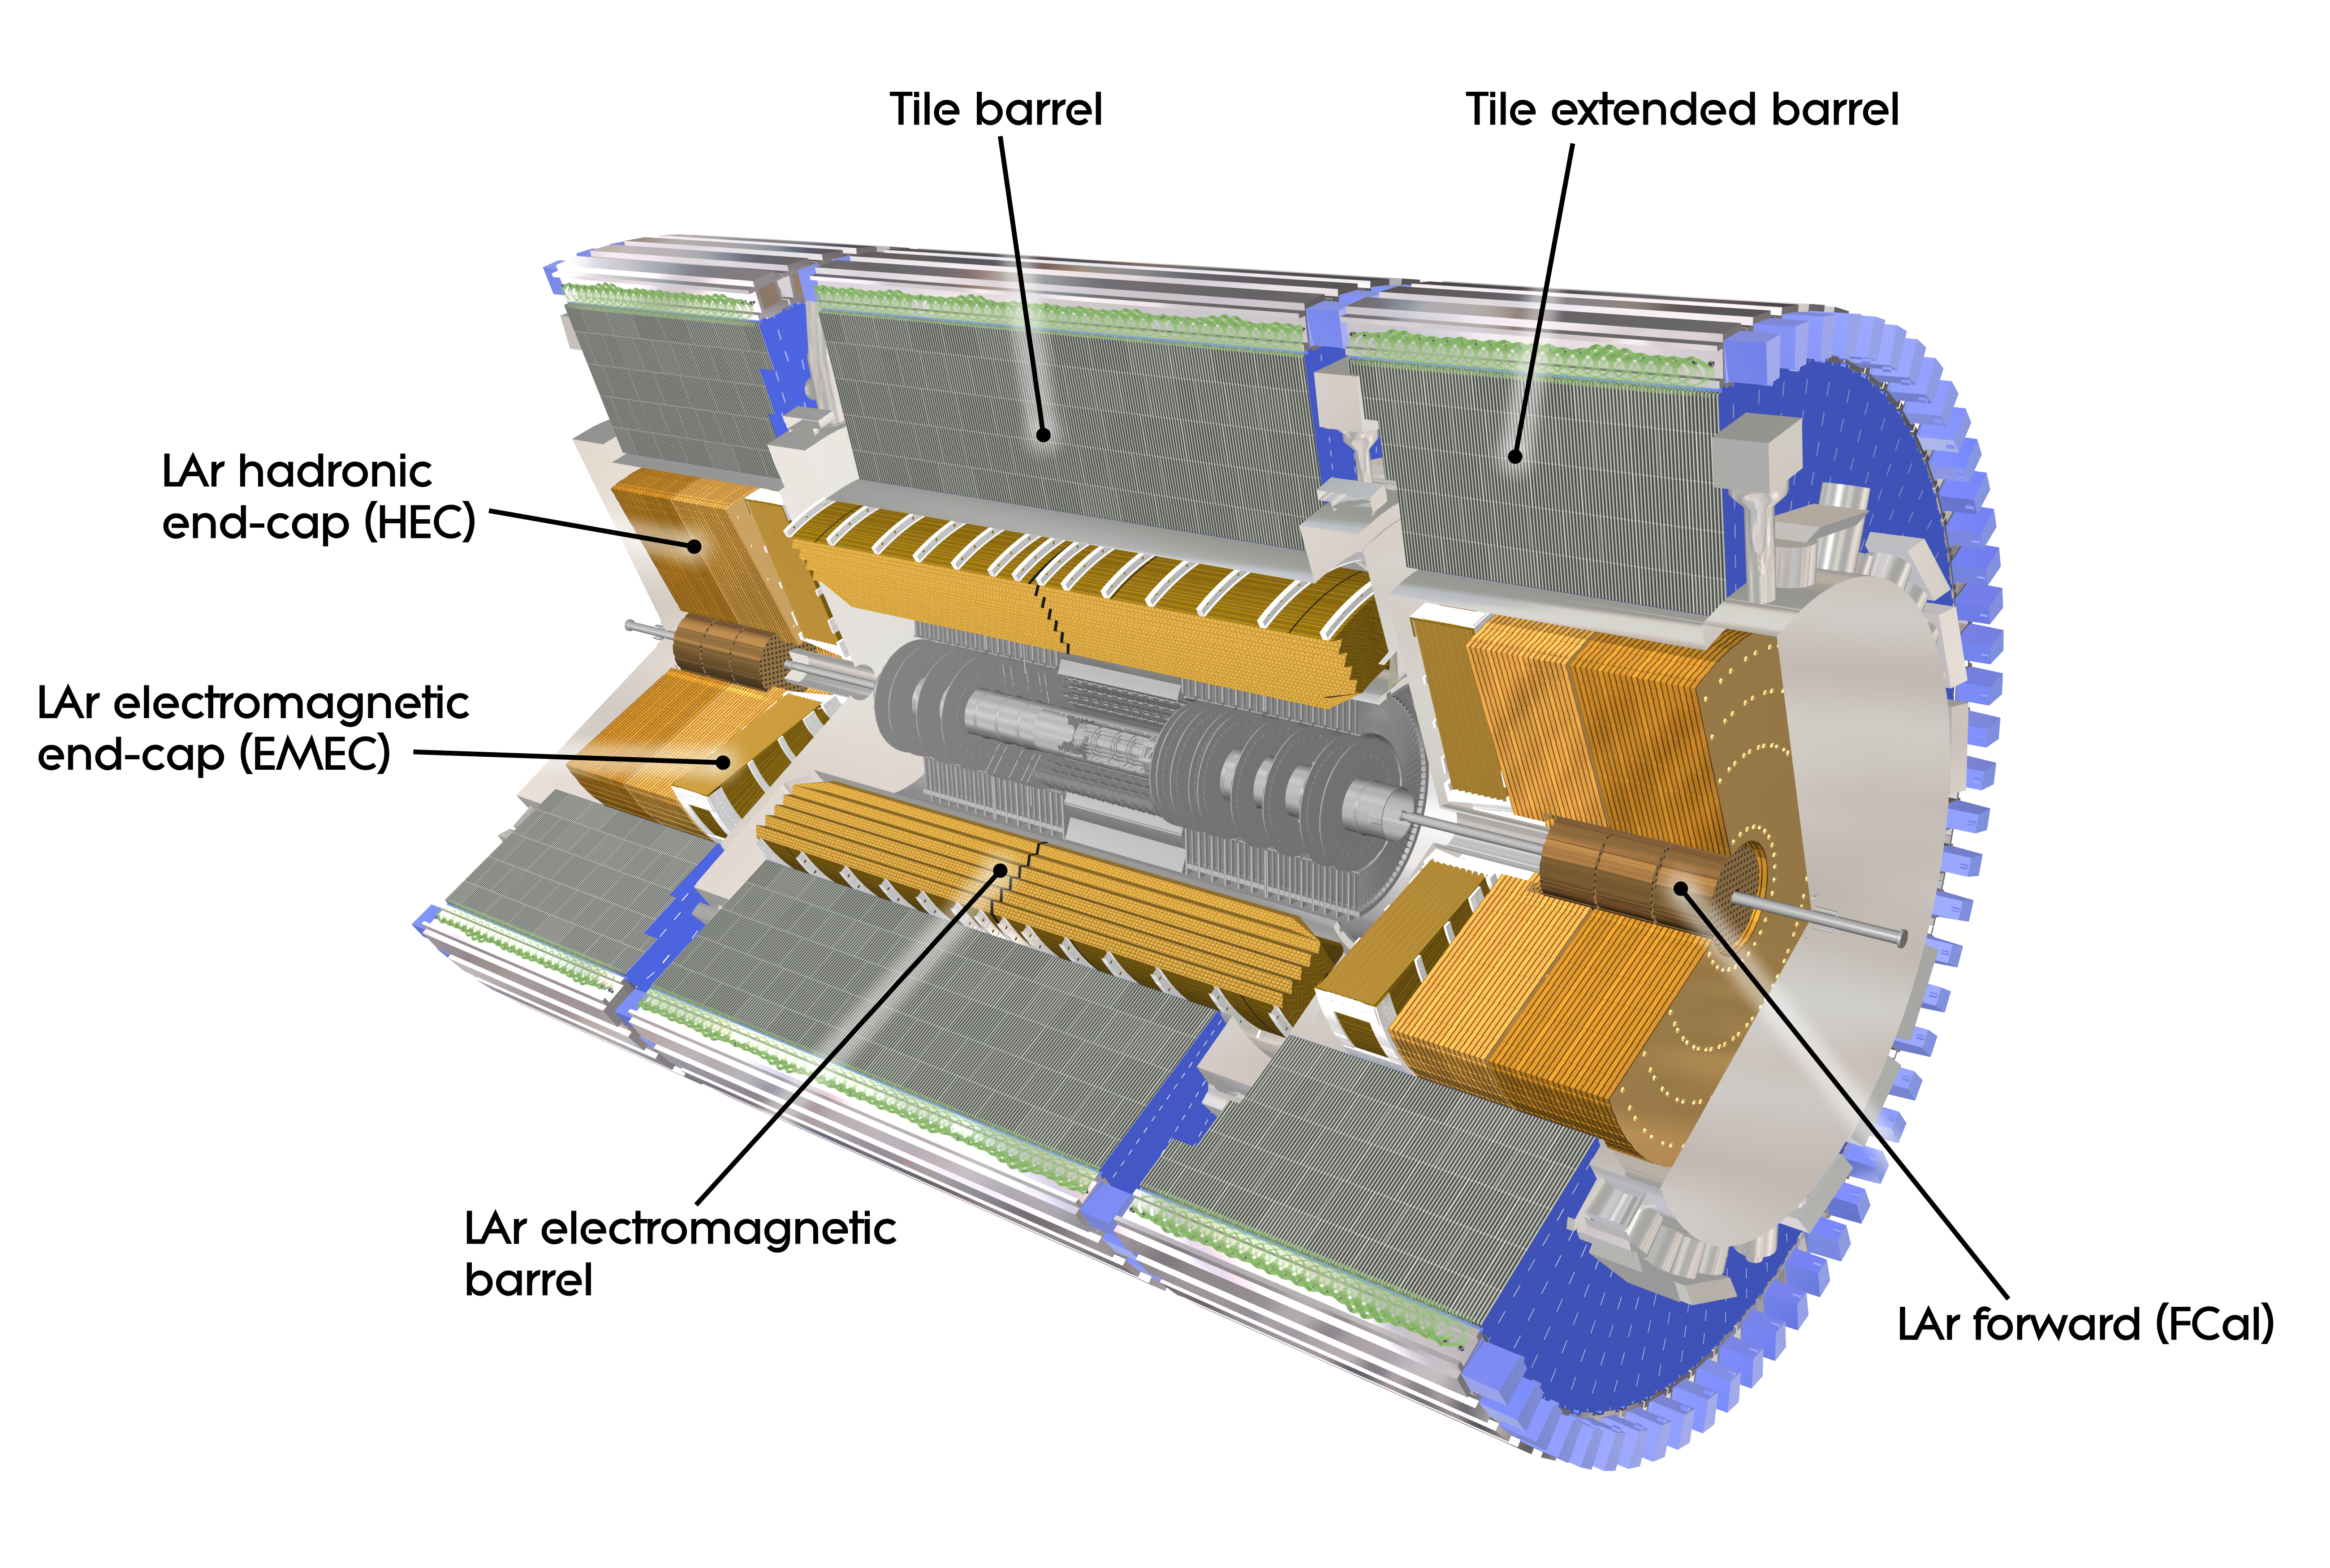
\includegraphics[width=0.8\textwidth]{Images/atlas/CALO.jpg}
\caption{Cut-away view of the ATLAS calorimeter system}
\label{pic:calo}
\end{figure}

Over the |$\eta$| range where the calorimeter is surrounding the ID, the EM calorimeter is finely segmented for precision measurements of electrons and photons, while the rest of the calorimeter is segmented more coarsely since it is mainly aimed at reconstructing jets and at measuring the missing transverse momentum.\\
Another important design criterion was the need of containing electromagnetic and hadronic showers of particles of energies around the TeV scale, since energy escaping the calorimeter results both in a significantly reduced energy resolution and in punch-through into the muon system. The total thickness of the EM calorimeter is 22~X$_0$ in the barrel and 24~X$_0$ in the end-caps.
Another important parameter to characterize the calorimeters is the absorption length $\lambda$. This is defined as distance into a material when the probability has dropped to 1/e that a particle has not been absorbed. The absorption length is typically used to describe the hadronic interaction of particles with the material.
The approximately 10 absorption length both in the barrel and in the end-caps are sufficient to provide very good resolution for high energy jets. The total thickness, including the outer support, is 11 $\lambda$ at |$\eta$|=0; this has been shown by simulation and confirmed by test beam data to be sufficient to reduce punch-throughs into the muon system well below the irreducible level of prompt or in-flight decays into muons.
The pseudo-rapidity coverage, granularity and segmentation is depth of the calorimeters are summarized in table \ref{tab:calo}

\begin{table}
\center
\begin{tabular}{l|lr|lr}
\hline
																			& \multicolumn{2}{c}{Barrel} 											& \multicolumn{2}{c}{End-cap}	\\ %				& Run II initial paramaters \\
\hline
\multicolumn{5}{c}{\tiny{EM calorimeter}} \\
\hline
\multicolumn{5}{c}{\tiny{Numbers of Layers and $|\eta|$ coverage}} \\
\hline
Presampler 													& 1 & |$\eta$| < 1.52& 2 & 1.5 < |$\eta$| < 1.8 \\
\hline
Calorimeter 												& 3 & |$\eta$| < 1.35& 2 & 1.375 < |$\eta$| < 1.5 \\
					 													& 2 & 1.35 <|$\eta$| < 1.475 & 3 & 1.5 < |$\eta$| < 2.5 \\
					 													&		&												& 2 & 2.5 < |$\eta$| < 3.2 \\
\hline
\end{tabular}
\end{table}

\paragraph{Electromagnetic Calorimeter}

The Electromagnetic Calorimeter is divided into a barrel (|$\eta$|<1.475) and two end-caps (1.375<|$\eta$|<3.2). Each end-cap calorimeter is mechanically divided in tow coaxial wheels: an outer wheel covering the region 1.375<|$\eta$|<2.5 and an inner wheel covering 2.5<|$\eta$|<3.2. The EM calorimeter is based on a lead-LAr detector with accordion-shaped kapton electrodes and lead absorbed plates over its full coverage. The liquid argon was chosen as an active medium because of its intrinsic radiation hardness and good energy resolution. he advantage of the accordion geometry is that it provides complete $\phi$ symmetry without azimuthal cracks.
Over the region which is intended to be used for precision physics (|$\eta$|<2.5) the EM calorimeter is segmented in depth in three sections. In addition, a presampler is used to recover the energy lost in dead material in front of the calorimeter. The layout of the barrel is shown in Figure \ref{pic:emcalo}.

\begin{figure}
\center
\includegraphics[width=0.8\textwidth]{Images/atlas/EMCALO.jpg}
\caption{Sketch of a barrel module where the different layers are clearly visible with the ganging electrodes in $\phi$. The granularity in $\eta$ and $\phi$ of the cells of each of the three layers of the trigger towers is also shown.}
\label{pic:emcalo}
\end{figure}

The first layer of the calorimeter, called the $\eta$-strip layer, is finely granulated in $\eta$ in order to allow for a better separation between photons (which results in a single energy deposition) and neutral pions, which results into two very close deposits of energy (from the $\pi^0\rightarrow \gamma \gamma$ decay). The resolution achievable in the barrel EM calorimeter, according to test beam data, is:

\begin{equation}
\frac{\sigma (E)}{E} = \frac{10\%}{\sqrt{E(GeV)}} \oplus 0.17\%
\end{equation}

where 10\% is the stochastic term and 0.17\% is the constant term. The energy response is also linear within $\pm0.1\%$. Similar results have been obtained for the end-cap EM calorimeters.
At the transition between the barrel and the end-cap calorimeters, at the boundary between the two cryostats, the amount od material in front of the calorimeter reaches a localized maximum of about 7$X_0$. For this reason, the region $1.37<|\eta|<1.52$ is not used for precision measurements involving photons and electrons.

\paragraph{Hadronic Calorimeters}

The hadronic calorimeters are subdivided in the tile calorimeter, whose barrel covers the region |$\eta$|<1.0 and whose extended barrels cover the region 0.8<|$\eta$|<1.7, in the LAr hadronic end-cap calorimeters, which extends from |$\eta$| = 1.5 up to |$\eta$| = 3.1 and finally the LAr forward calorimeter, which covers the pseudorapidity range up to |$\eta$| = 4.9. The tile calorimeter uses steel as the absorber and scintillating tiles as active material. Two sides of the scintillating tiles are read out by wavelength shifting fibres into two separate photomultiplier tubes. The energy response to isolated charged pions of the combined LAr and tile calorimeter was tested with test beam and turns out to be:

\begin{equation}
\frac{\sigma (E)}{E} = \frac{52\%}{\sqrt{E(GeV)}} \oplus 3\%
\end{equation}

For the end-cap hadronic calorimeters LAr technology is used, analogously to the EM calorimeter in the barrel region, but copper is used instead of lead as a passive material and a flat-late geometry was chosen. The energy response to isolated pions can be condensed in the energy resolution:

\begin{equation}
\frac{\sigma (E)}{E} = \frac{71\%}{\sqrt{E(GeV)}} \oplus 1.5\%
\end{equation}

Finally, the forward calorimeter is based again on LAr active material and uses copper as passive absorber material for the first layer and tungsten for the second and third layer. As a result of test beam data the energy response to pions is expressed by the relative energy resolution:

\begin{equation}
\frac{\sigma (E)}{E} = \frac{94\%}{\sqrt{E(GeV)}} \oplus 7.5\%
\end{equation}



\subsubsection{Muon System}

The detection of muons in ATLAS can count on a dedicated sub-detector. Muons are among the most important signatures for interesting processes at the LHC and have a clear advantage that they are the only charged particles which are not stopped in the calorimeter (apart rare cases of punch-through) and they are detected in the muon system. This can be exploited also for the on-line selection of events.
The muon detector is based on two kind of sub-detectors, one for precision measurements, which is needed to determine the muon momenta with high precision, and another for the online trigger of muon events, which requires very fast sub-detectors and are needed to uniquely associate the muons to a certain bunch crossing. The precision measurements are performed by the Monitored Drift Tube chambers (MDT), which cover the pseudorapidity region up to 2.7, and, in the forward region (2<|$\eta$|<2.7), by Cathode-Strip Chambers (CSC), which are used in the innermost layer due to their capability of working at high rate and better time resolution.
The MDT chambers only constrain the muon track in the bending plane (z-coordinates), with a precision of \SI{35}{\micro\meter}, while the CSC, being multi-wire proportional chambers with cathode planes segmented into strips in orthogonal direction, provide a measurement both in the R direction of \SI{40}{\micro \meter} precision and in the $\phi$ direction of \SI{10}{\milli\meter}.
These chambers are complemented (both for the measurement of the missing $\phi$ in case of the MDT and for the online event selection) in the barrel region (|$\eta$|<1.05) by Resistive Plate Chamber (RPC) and in the end-cap (1.05<|$\eta$|<2.4) by Thin Gap Chambers (TGC). The intrinsic time resolution of these detectors components (\SI{1.5}{\nano\second} for RPC and \SI{4}{\nano\second} for TGC) is appropriate for triggering and permits to identify the correct bunch crossing.\\
Given the three chambers layout of the muon system, the momentum measured of a high-\pt track will depend on the resolution by which its sagitta (determined in the R-z plane in the middle chamber with respect to a straight line) can be determined. For high-pt track of \SI{1}{\TeV}, this sagitta will be about the \SI{500}{\micro \meter}. The muon chamber resolution provided in $\phi$ by the MDT chambers allows to reach a precision better than 10\% in the momentum measurements of muons up to \SI{1}{\TeV}, which corresponds to the design goals of ATLAS.
For the measurements of low-\pt muons, the measurements in the muon system typically need to be complemented by measurements in the ID, since in general not all muon stations will be reached due to the stronger bending of low-\pt particles in the magnetic field.

\subsubsection{Trigger System}

The ATLAS experiment uses a two staged trigger system to identify collisions events of interest.\\
The first stage, called Level-1 trigger, reduces the event rate from \SI{40}{\mega\hertz} to \SI{100}{\kilo\hertz},
since a decision must be taken every \SI{25}{\nano\second}. Since the transit and processing time of around \SI{2.5}{\micro\meter}, the detector data must be time stamped and held in the buffers of the front-end circuit.
The Level-1 trigger uses information from dedicated muon trigger and from the calorimeters. The only signatures which can be selected in the L1 trigger are high-\pt muons, electrons/photons, jets, $\tau$-lepton decaying into hadrons and missing transverse energy. No information coming from the tracking devices can be used at L1, so, for example, it is not possible to select b-jets at this level.\\
The second stage of the trigger system reduces the event rate further \SIrange{0.5}{1}{\kilo\hertz}. It is software based and uses offline-like reconstruction algorithms, utilizing informations from all sub-detectors in regions of interest around the Level-1 objects in full granularity. The regions of interest are areas of the detector which the L1 trigger has identified as interesting. The use of regions of interest allows to have a fast execution time keeping high the selection efficiency.

%The L2 and EF triggers form the High-Level Trigger (HLT) and are both based on commercially available computer and networking hardware. The main difference between the L2 and the EF is that the first is seeded by so-called Regions-of-Interests (RoI), which are regions of the detector which the L1 trigger has identified as interesting, while the second is based on full-detector-granularity. In this way the L2 trigger is much quicker and yields a first rate reduction from $75~kHz$ to below $3.5~kHz$, with an average processing time of approximately $40~ms$, while the EF brings this further down to $200~Hz$, with a processing time per event of around 4 seconds. The higher granularity, tracking information and improved reconstruction make a refined decision with respect to the L1 possible. The final rate can be sustained by actual storage technology.

\subsection{The LHC upgrade program}

\begin{figure}
\center
\subfloat[2011 Luminosity]{\label{pic:atlaslumi2011}\includegraphics[width=0.45\textwidth]{Images/atlas/ATLASLUMIRUN1_2011.png}}\quad
\subfloat[2012 Luminosity]{\label{pic:atlaslumi2012}\includegraphics[width=0.45\textwidth]{Images/atlas/ATLASLUMIRUN1_2012.png}}
\caption{Cumulative luminosity versus day, in green the amount of luminosity deliverd to ATLAS and in yellow the recorderd one. This assume stable beam configuration for proton-proton collisions.}
\label{pic:atlaslumi}
\end{figure}
The LHC machine and the related experiments showed excellent performance in the first run period of the LHC, which took place in between 2010 and 2012, delivering almost \SI{30}{\per\femto\barn} to the ATLAS and CMS experiments. The ATLAS experiment was able to record 93$\percent$ of the delivered luminosity as shown in Figure \ref{pic:atlaslumi} for what concerns the proton-proton collisions.

\begin{figure}
\center
\includegraphics[width=0.9\textwidth]{Images/atlas/ATLASSM.png}
\caption{Detailed summary of several Standard Model total production cross section measurements, corrected for leptonic branching fractions, compared to the corresponding theoretical expectations. All theoretical expectations were calculated at NLO or higher. The W and Z vector-boson inclusive cross sections were measured with \SI{35}{\per\pico\barn} of integrated luminosity from the 2010 dataset. All other measurements were performed using the 2011 dataset or the 2012 dataset. The dark-color error bar represents the statistical uncertainly. The lighter-color error bar represents the full uncertainty, including systematics and luminosity uncertainties.}% The data/theory ratio, luminosity used and reference for each measurement are also shown. Uncertainties for the theoretical predictions are quoted from the original ATLAS papers. They were not always evaluated using the same prescriptions for PDFs and scales. For the dijets measurement, $y^* = |y_1 - y_2|/2$, where $y_i$ is the jet rapidity. }
\label{pic:atlassm}
\end{figure}

Detailed measurements of well-known SM processes were performed and used to calibrate the detector. Figure \ref{pic:atlassm} shows the measured production cross section for several SM processes with their theoretical prediction. 
The success of the discovery of the Higgs Boson was just one of the impressive results achieved by LHC experiments during the first period of data-taking. Further investigation on the Higgs boson properties and in the search of new physics phenomena will require to collect more data; therefore the LHC luminosity need to increase and the detectors performance need to improve. An increase of the center of mass energy will allow to explore a more wide phase space of physics phenomena.\\
\begin{figure}
\centering
\includegraphics[width=0.9\textwidth]{Images/atlas/LHC_upgrade_program.png}
\caption{Time schedule for the long LHC shutdowns and the run phases}
\label{pic:lhc_schedule}
\end{figure}
Figure~\ref{pic:lhc_schedule} summarizes the upgrade steps of the LHC machine. A first long shutdown happened from February 2013 to April 2015 to consolidate the magnet inter-connects of the LHC machine. This upgrade was needed to run the LHC at the design energy of \SI{7}{\TeV} per beam and at the design luminosity of \SI{e34}{\per\square\centi\meter\per\second}. The period after such an upgrade of the LHC is usually referred as Run 2, and it should last from 2015 to 2019, aiming to collect \SI{100}{\per\femto\barn} of data. The Run 2 has began in the spring of 2015, with a \SI{13}{\TeV} center of mass energy, which will be upgraded to \SI{14}{\TeV} in next years.
A second and a third shutdown with machine development are foreseen in 2019 and 2024, where the luminosity should be upgraded to twice and five times the nominal value.
The LHC plan is to record about \SI{3000}{\per\femto\barn} during the entire LHC data-taking campaign.\\
The LHC upgrades provide the opportunity to upgrade the experiments and to recover possible failures.
The first long shutdown was used for an upgrade of the ATLAS pixel detector as it will be discussed in Chapter 3 of this thesis. While no upgrade of the ATLAS Pixel detector is foreseen in the second long shutdown a complete redesign will be needed after the third long shutdown. The new system should in particular sustain the harsh radiation environment and provide fast information for the new track based trigger system.
%\subsection{Physics with b-tagging in the LHC Run 2}
%The identification of jets containing b hadrons is an important tool used in a spectrum of measurements comprising the Large Hadron Collider (LHC) physics programme. In precision measurements in the top quark sector as well as in the search for the Higgs boson and new phenomena, the suppression of background processes that contain predominantly light-flavour jets using b-tagging is of great use. It may also become critical to achieve an understanding of the flavour structure of any new physics (e.g. supersymmetry) revealed at the LHC.
%Several algorithms to identify jets containing b hadrons have been developed, exploiting the
%long lifetime, high mass and decay multiplicity of b hadrons and the hard b-quark fragmentation
%function. They range from an algorithm that uses the signed significance of the decay length with
%respect to the proton-proton collision location, in the following referred to as the primary vertex,
%of an inclusively reconstructed secondary vertex to more refined algorithms using both secondary
%vertex properties and the significance of the transverse and longitudinal impact parameters of the
%charged particle tracks. The most discriminating variables resulting from these algorithms are
%combined in artificial neural networks. An independent b-tagging algorithm based on reconstructed
%muons inside jets, exploiting the relatively large fraction of b-hadron decays with muons in the
%final state, about $20\percent$, and the b-tagging algorithm used for the online trigger selection are also used.
%The performance of the tagging algorithms is studied in simulated events, including the dependence on additional proton-proton interactions in the same bunch crossing, referred to as pile-up.


\pagebreak
